\section{Design}
\label{s:design}

\begin{figure*}
  \centering
  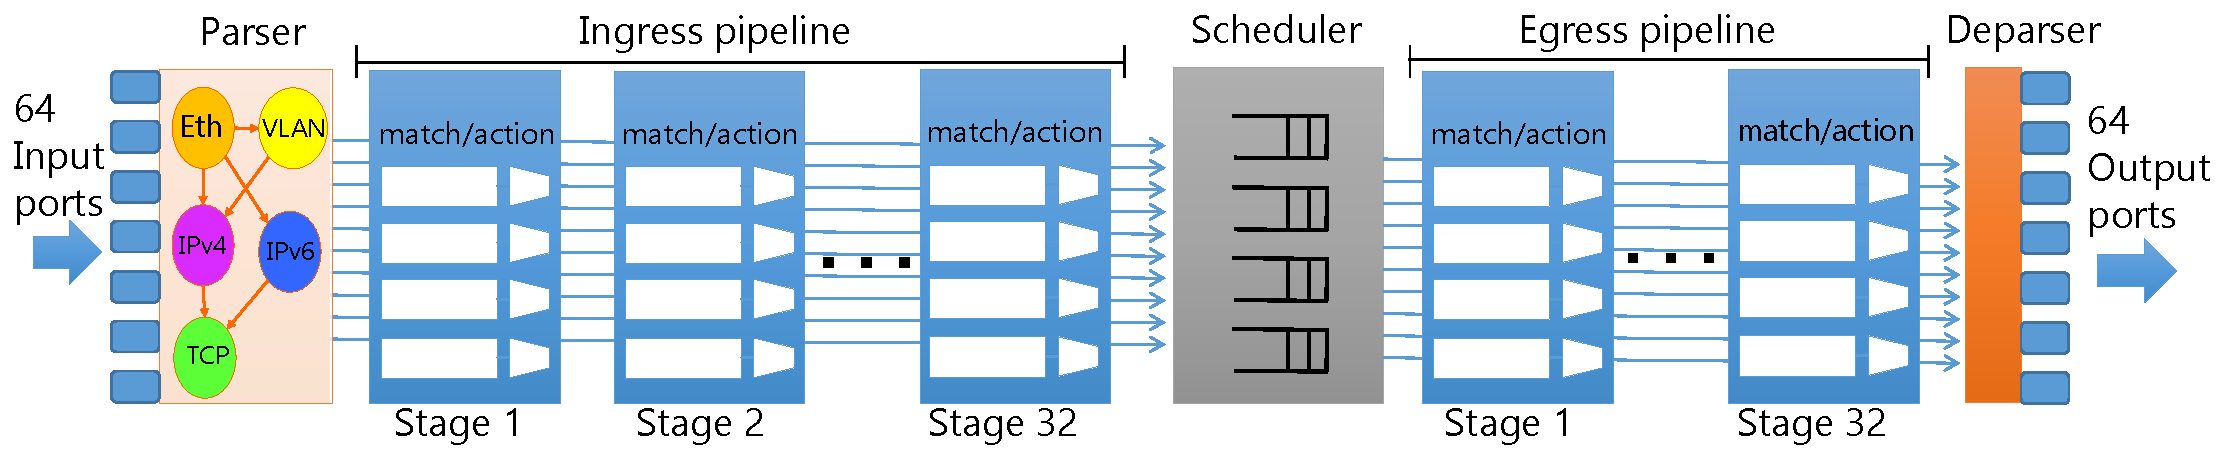
\includegraphics[width=\textwidth]{pifo_router_pipeline.pdf}
  \caption{A shared memory router.  Combinational logic and memory are
  shared across ports, both in the pipelines and in the scheduler.}
%The router runs at a clock frequency of 1 GHz.}
  \label{pifo_fig:router}
\end{figure*}

We now present a hardware design for a programmable scheduler based on PIFOs.
We target shared-memory routers such as Broadcom's Trident II~\cite{trident2}
(Figure~\ref{pifo_fig:router}). In these routers, a parser feeds packets from
all ports into a shared ingress pipeline, after which they enter a shared
scheduler and a similarly shared egress pipeline. To reduce chip area,
combinational logic and memory for packet processing are shared across ports,
both in the pipelines and in the scheduler. As discussed earlier
(\S\ref{s:absmachine}), the number of pipelines depends on the aggregate
capacity of the router. For our PIFO design, we focus on a 64-port 10G
single-pipeline router, where one pipeline handles the aggregate processing
requirements of all ports at minimum packet size, \ie 64 10 Gbit/s ports each
transmitting 64 byte packets. This translates into \textasciitilde 1 billion
packets per second, after accounting for minimum inter-packet gaps, or a 1 GHz
clock frequency.

We first describe how scheduling and shaping transactions can be implemented
(\S\ref{ss:transactions}). Then, we show how a tree of PIFOs can be realized
using a full mesh of {\em PIFO blocks} by appropriately interconnecting these blocks
(\S\ref{ss:mesh}). We also describe how a compiler (\S\ref{pifo_ss:compiler}) could
automatically configure this mesh from a scheduling tree.

\subsection{Scheduling and shaping transactions}
\label{ss:transactions}
To program and implement scheduling and shaping transactions, we use Domino
(Chapter~\ref{chap:domino}). Domino allows us to express these transactions in
Domino's domain-specific language, using a compiler to compile the transactions
down to a pipeline of \absmachine atoms.  One of the examples used to evaluate
Domino in \S\ref{s:eval} is the STFQ transaction from
Figure~\ref{fig:sched_trans}.  Specifically, Table~\ref{tab:algos} shows that
the STFQ transaction can be run at 1 GHz on a router pipeline with the Pairs
atom.

%TODO: We need to evaluate this more thoroughly.
Similarly, we could use the Domino compiler to compile other scheduling and
shaping transactions to an atom pipeline.  For example, the transactions for
Token Bucket Filtering (Figure ~\ref{fig:hshaping_shaping_trans}), minimum rate
guarantees (\S\ref{ss:min_rate}), Stop-and-Go queueing (\S\ref{ss:stopngo}),
and LSTF (\S\ref{ss:lstf}), can all be expressed as Domino programs. They can
then be compiled to a router pipeline with a sufficiently expressive
atom. An important restriction in Domino is the absence of loops, which
precludes rank computations containing a loop with an unbounded iteration
count. We have not, however, encountered a scheduling or shaping transaction
requiring this capability.
% Loops with bounded iteration count can be unrolled.

\begin{figure}[!t]
  \centering
  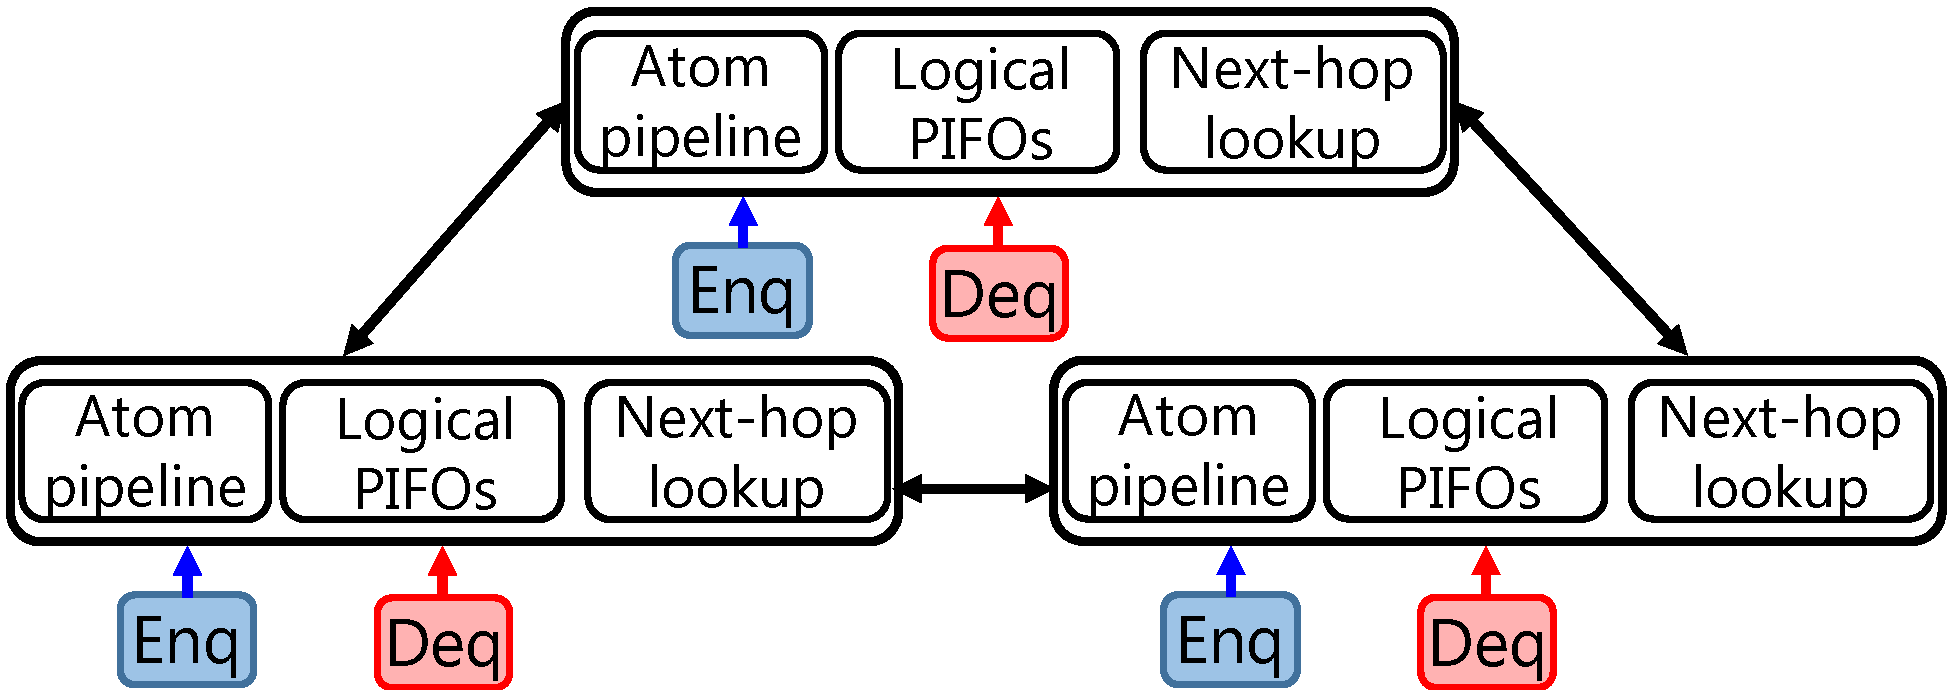
\includegraphics[width=0.6\columnwidth]{pifo_pifo_mesh.pdf}
  \caption{Three PIFO blocks in a PIFO mesh}
  \label{fig:mesh}
\end{figure}

\begin{figure}[!t]
  \centering
  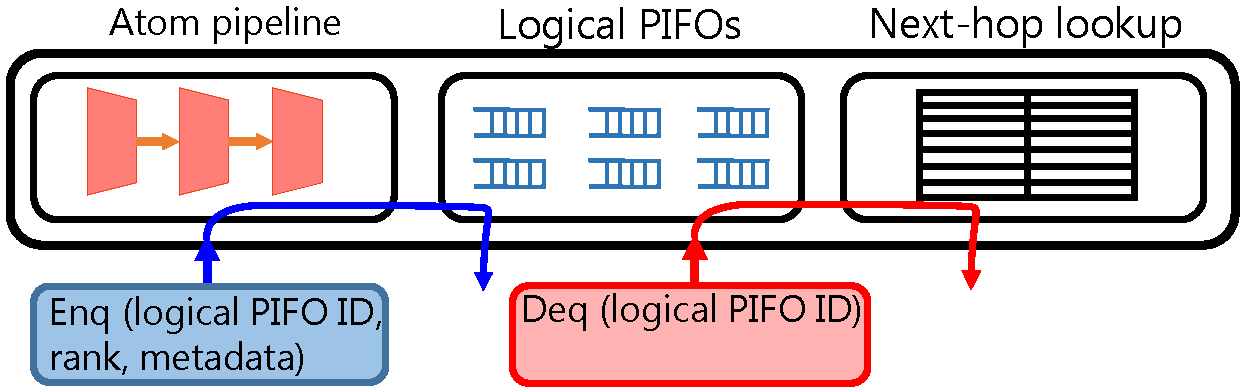
\includegraphics[width=0.6\columnwidth]{pifo_pifo_block.pdf}
  \caption{A single PIFO block. Enqueue operations execute transactions in the atom pipeline
  before enqueuing elements into a logical PIFO. Dequeue operations dequeue elements from logical PIFOs
  before looking up their next hop.} 
  \label{fig:block}
\end{figure}

\begin{figure*}[!t]
  \begin{subfigure}[b]{0.5\textwidth}
  \begin{center}
  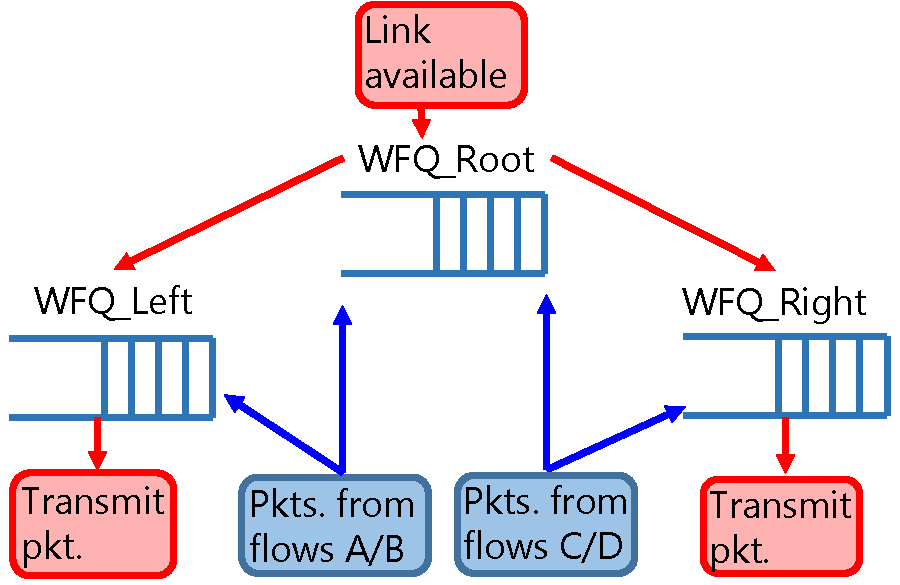
\includegraphics[width=\textwidth]{pifo_hpfq_logical.pdf}
  \caption{Logical PIFO tree for HPFQ}
  \label{fig:hpfq_path}
  \end{center}
  \end{subfigure}
  \begin{subfigure}[b]{0.5\textwidth}
  \begin{center}
  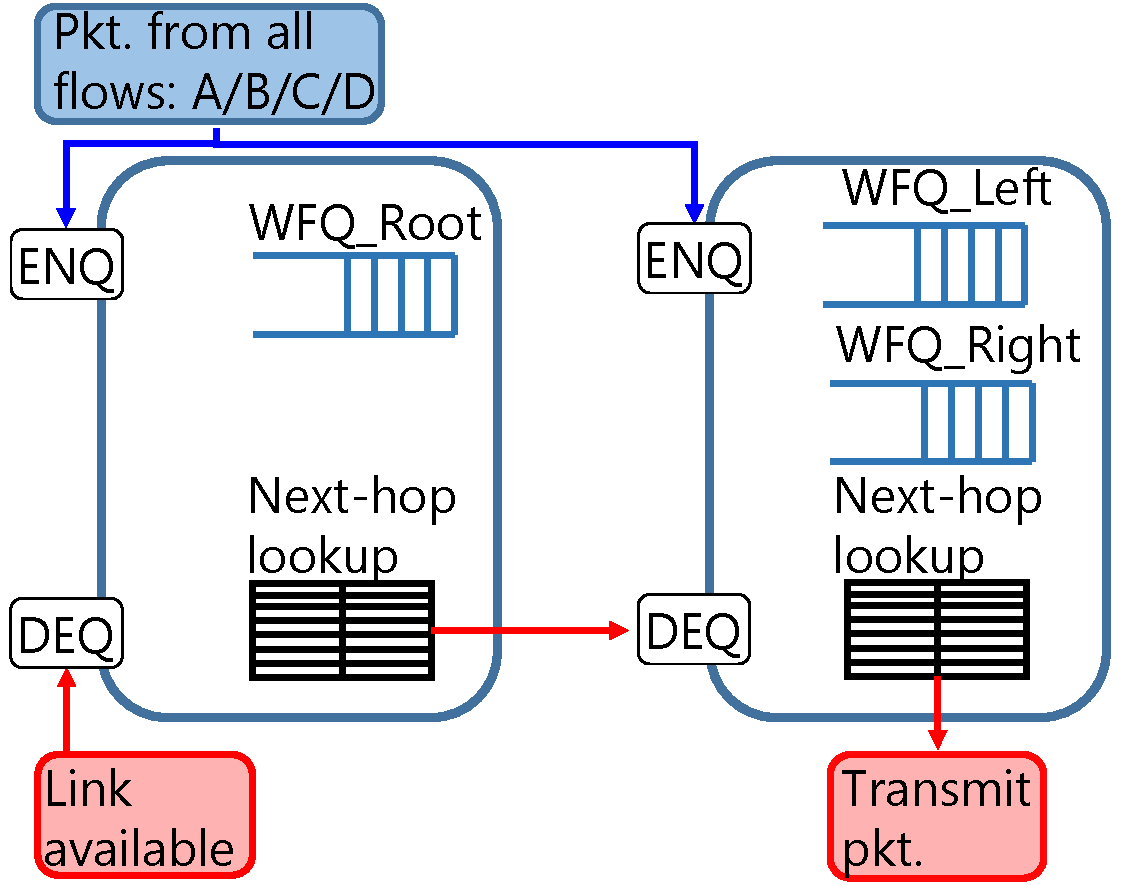
\includegraphics[width=0.8\textwidth]{pifo_hpfq_physical.pdf}
  \caption{Physical PIFO mesh for HPFQ}
  \label{fig:hpfq_mesh}
  \end{center}
  \end{subfigure}
  \caption{Compiling HPFQ (Figure~\ref{fig:hpfq}) to a PIFO mesh. On the left,
  the logical PIFO tree captures relationships between PIFOs: which PIFOs dequeue
  or enqueue into which PIFOs. Red arrows indicate dequeues, blue indicates
  enqueues.  On the right, we show the physical PIFO mesh for the logical PIFO
  tree on the left, following the same notation.}
  \label{fig:hpfq_compiling}
\end{figure*}

% Hopefully, this bit below they should have understood from earlier.
% All packets result in two enqueues: to the root
%  PIFO and one of the two leaf PIFOs. This is shown using two arrows starting
%  from one point (\eg the arrows originating from A/B).

\begin{figure*}[!t]
  \begin{subfigure}[b]{0.5\textwidth}
  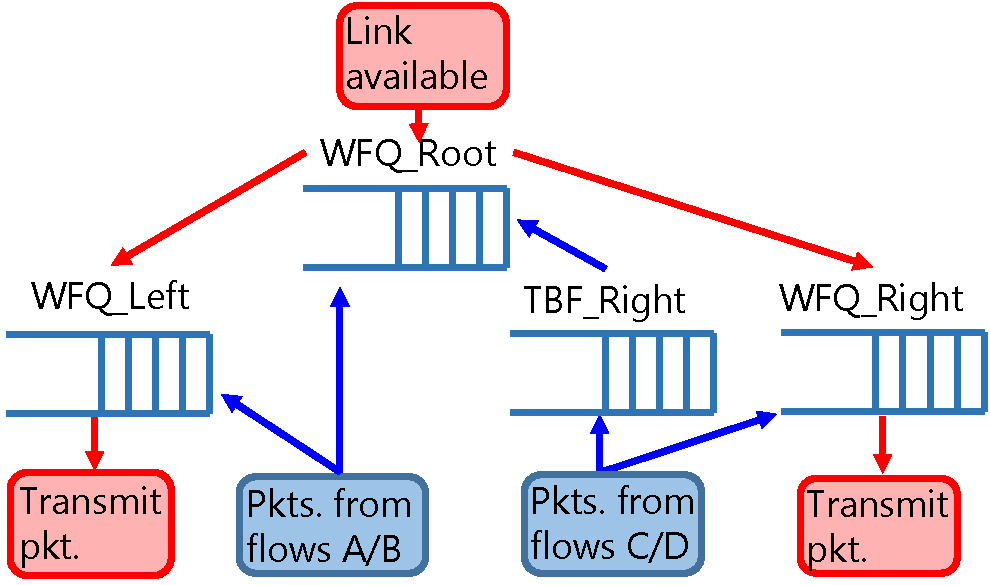
\includegraphics[width=\textwidth]{pifo_hshaping_logical.pdf}
  \caption{Logical PIFO tree for Hierarchies with Shaping}
  \label{fig:hshaping_path}
  \end{subfigure}
  \begin{subfigure}[b]{0.5\textwidth}
  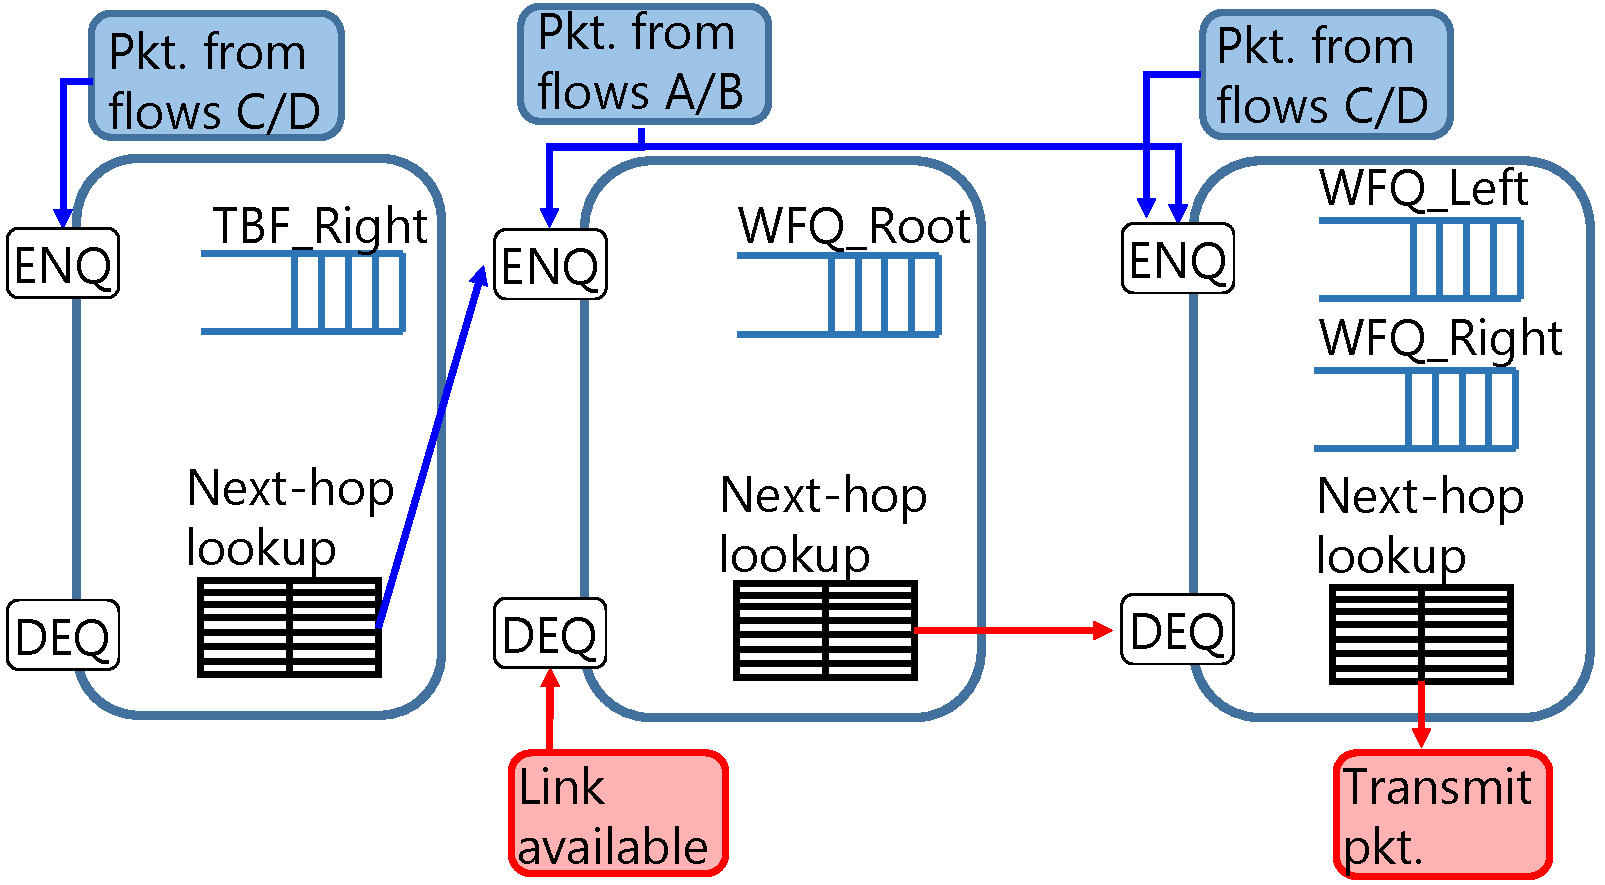
\includegraphics[width=\textwidth]{pifo_hshaping_physical.pdf}
  \caption{Physical PIFO mesh for Hierarchies with Shaping}
  \label{fig:hshaping_mesh}
  \end{subfigure}
  \caption{Compiling Hierarchies with Shaping (Figure~\ref{fig:hpfq}) to a PIFO mesh. Same comments as Figure~\ref{fig:hpfq_compiling} apply.}
\end{figure*}


\subsection{The PIFO mesh}
\label{ss:mesh}

%TODO: Define logical PIFO before.
We lay out PIFOs physically as a full mesh (Figure~\ref{fig:mesh}) of
{\em PIFO blocks} (Figure~\ref{fig:block}). Each PIFO block supports
multiple logical PIFOs. These logical PIFOs correspond to PIFOs for
different output ports or different classes in a
hierarchical scheduling algorithm, which share the combinational logic
required for a PIFO. We expect a small number of PIFO blocks in a
typical router (\eg fewer than five) because each PIFO block
corresponds to a different level of a hierarchical scheduling tree and
most practical hierarchical scheduling algorithms we know of do
  not require more than a few levels of hierarchy. As a result, a
full mesh between these blocks is feasible (\S\ref{ss:interconnect}
has more details).

% Maybe subsection for a PIFO block?
PIFO blocks run at 1 GHz and contain an atom
pipeline to execute scheduling and shaping transactions before enqueuing into a
logical PIFO. In every clock cycle, each PIFO block supports one enqueue and
dequeue operation on a logical PIFO residing within that block
(shaping transactions require more than one operation per clock cycle and
are discussed in \S\ref{ss:shape_challenge}). We address a logical PIFO within
a block with a logical PIFO ID.

The interface to a PIFO block is:
\begin{CompactEnumerate}
\item Enqueue an element (packet or reference to another PIFO) given a
  logical PIFO ID, the element's rank, and some metadata that will be
  carried with the element such as the packet length required for
  STFQ's rank computation. The enqueue returns nothing.
\item Dequeue from a specific logical PIFO ID within the block. The dequeue
   returns either a packet or a reference to another PIFO.
\end{CompactEnumerate}

After a dequeue, besides transmitting a packet, a PIFO block may
communicate with another PIFO block for two reasons:
 \begin{CompactEnumerate}
 \item To dequeue a logical PIFO in another block, \eg when dequeuing a
   sequence of PIFOs from the root to a leaf of a scheduling tree to transmit
   packets.
 
 \item To enqueue into a logical PIFO in another block, \eg when
   enqueuing a packet that has just been dequeued from a shaping
   PIFO.
 \end{CompactEnumerate}

We configure these post-dequeue operations using a small lookup table, which
looks up the ``next hop'' following a dequeue. This lookup table specifies an
operation (enqueue, dequeue, transmit), the PIFO block for the next operation,
and any arguments the operation needs.

\subsection{Compiling from a scheduling tree to a PIFO mesh}
\label{pifo_ss:compiler}

\an{A programmer should not have to manually configure a PIFO mesh. Instead, a
compiler translates from a scheduling tree to a PIFO mesh configuration implementing that tree.  While we haven't prototyped
this compiler, we illustrate how it would work using HPFQ (Figure~\ref{fig:hpfq})
and Hierarchies with Shaping (Figure~\ref{fig:hshaping}).}

The compiler first converts the scheduling tree to a logical PIFO tree that
specifies the enqueue and dequeue operations on each PIFO.
Figures~\ref{fig:hpfq_path} and \ref{fig:hshaping_path} show the logical PIFO tree for
the scheduling trees in Figures~\ref{fig:hpfq} and \ref{fig:hshaping} respectively.  It then overlays
this tree over a PIFO mesh by assigning every level of the tree to a PIFO block
and configuring the lookup tables to connect PIFO blocks as required by the
tree.  Figure~\ref{fig:hpfq_mesh} shows the PIFO mesh for
Figure~\ref{fig:hpfq}, while Figure~\ref{fig:hshaping_mesh} shows the PIFO mesh
for Figure~\ref{fig:hshaping}.

If a particular level of the tree has more than one enqueue or dequeue from
another level, which \an{arises in the presence of shaping transactions
(\S\ref{ss:shape_challenge})}, we allocate new PIFO blocks to respect the
constraint that any PIFO block provides only one enqueue and dequeue operation per
clock cycle, \eg Figure~\ref{fig:hshaping_mesh} has an additional PIFO block
containing TBF\_Right alone. Finally, we use the Domino compiler to compile
scheduling and shaping transactions.
%%
%%\footnote{More precisely, the shaping PIFO that the TBF\_Right
%%transaction enqueues into. We use a transaction's name to refer both to the
%%transaction and the PIFO it enqueues into.} 
%TODO: Could make above paragraph a bit more lucid.

\subsection{Challenges with shaping transactions}
\label{ss:shape_challenge}

Each PIFO block supports one enqueue and dequeue operation per clock cycle.
This suffices for any algorithm that only uses scheduling transactions
(work-conserving algorithms) because, for such algorithms, each packet needs at
most one enqueue and one dequeue at each level of its scheduling tree, and we
map the PIFOs at each level to a different PIFO block.

However, shaping transactions pose challenges. Consider Hierarchies with
Shaping (Figure~\ref{fig:hshaping_path}). When the shaping transaction enqueues
elements into TBF\_Right, these elements will be released into WFQ\_Root at a
future time $T$. The external enqueue into WFQ\_Root may also happen exactly at
$T$, if a packet arrives at $T$. This creates a conflict because there are two
enqueue operations in the same cycle.  Conflicts may also occur on dequeues.
For instance, if TBF\_Right shared its PIFO block with another logical PIFO,
dequeue operations to the two logical PIFOs could occur at the same time
because TBF\_Right can be dequeued at any arbitrary wall-clock time.

%%\MA{I think a transient variant of this problem exists with scheduling
%%  transactions as well if the PIFOs for different ports are not
%%  carefully placed. For example, if the WFQ\_Root PIFO for port 1 is in the
%%  same block as the WFQ\_Right PIFO for port 0, there could be a
%%  conflict. The difference (I think) is that this one is transient; it
%%  can't affect things by more than N clock cycles if there are N
%%  ports, so it wouldn't affect the line rate. We don't need to explain
%%  this, unless anyone else also wondered about this}

In a conflict, only one of the two operations can proceed. We resolve
this conflict in favor of scheduling PIFOs. Shaping PIFOs are used for
rate limiting to a rate lower than the line rate. Therefore, they
can afford to be delayed by a few clocks until there are no
conflicts. By contrast, delaying scheduling decisions of a scheduling PIFO
would mean that the router would idle and not satisfy its line-rate guarantee.


As a result, shaping PIFOs only get best-effort
service. There are workarounds to this. One is overclocking the pipeline at
(say) 1.25 GHz instead of 1 GHz, providing spare clock cycles for such
best-effort processing. Another is to provide multiple ports to a PIFO block to
support multiple operations every clock.  These techniques are commonly used in
routers for background tasks such as reclaiming buffer
space, and can be applied to the PIFO mesh as well.
% Amy wondered if there would be other kinds of conflicts, i.e., shaping-shaping or scheduling-scheduling
